\documentclass{ximera}

\title{Algebra Sample Problems}
\author{Christine Lien}

%\voffset = 0 in
\usepackage{epsf,eurosym,amsmath,amssymb, graphicx, verbatim}
%\usepackage{enumerate}
\usepackage{alphalph}
\usepackage{pgffor}
\usepackage{stmaryrd}
\usepackage{tabularx}
%\usepackage{tabulary}

%\usepackage{pgfplots}
%\pgfplotsset{compat=newest}

%\setlength{\textwidth}{6.5in}
%\setlength{\oddsidemargin}{-.1in}
%\setlength{\evensidemargin}{-.3in}
%\setlength{\textheight}{9.0in}
%\setlength{\topmargin}{-.3in}
%\setlength{\unitlength}{.75truein}


%\newcommand{\PSbox}[3]{\mbox{\rule{0in}{#3}\special{psfile=#1}\hspace{#2}}}
%\renewcommand{\theenumii}{\alphalph{\value{enumii}}}
%\renewcommand{\theenumi}{\value{enumi}}

\setlist[enumerate, 1]{label=\arabic*.)}

\newcommand{\usualgrid}[4]{
  axis lines=middle,
  xlabel=$$,
  xlabel style={at=(current axis.right of origin), anchor=west},
  ylabel=$$,
  ylabel style={at=(current axis.above origin), anchor=south},
  xmin=#1,
  xmax=#2,
  ymin=#3,
  ymax=#4,
  xtick={#1,...,#2},
  ytick={#3,...,#4},
  xticklabels={,,},
  yticklabels={,,},
  grid=major,
}
\begin{document}



\hfill Math 112 

{\large\bf Exam 2 Sample Problems} 

\textit{Note: You must solve each problem using algebraic methods. Using trial and error will not be granted any credit.
\\
The problems here are just on material covered since Exam 1. Exam 2 is cumulative and the previous exam review will be relevant.}

\begin{enumerate}

\item List the 9 basic functions. 
\begin{enumerate}
\item Write down their domains, range, symmetry (if any), $x$ and $y$-intercepts (if they exist). \item Determine which of the 9 basic functions are 1-1. Justify your answer. If it is 1-1, find the inverse, the domain and range of the inverse, and sketch a graph of the inverse.  
\end{enumerate}

\item For each function $h(x)$ given below, decompose $f$ into the composition of two functions $f$ and $g$ so that $h(x)=(f\circ g)(x)$ and either $f$ or $g$ is one of the nine basic functions.
\begin{enumerate}
\item $h(x)=(x+5)^2$
\item $h(x)=\sqrt[3]{5x^2+1}$
\item $h(x)=\sqrt{x^2+6x+9}$
\item $\displaystyle h(x)= \frac{2}{x+5}$
\end{enumerate}


\item For the functions below, determine whether the function is 1-1. Justify your answer. If it is 1-1, find the inverse of the function, and the domain and range of the inverse. 

\begin{enumerate}
\item $f(x)=2x-1$.
\item $f(x)=3x^{2}+2$.
\item $\displaystyle f(x)=\frac{3x-1}{5x+2}$
\item $f(x)=(x-5)^{3}-8$
\item $\displaystyle f(x)=\frac{1}{2}|2x-1|+3$.
\item $f(x)=\sqrt{x-2}$.
\item Sketch a graph of the functions in (a), (b), (d), (e), and (f). If the functions have an inverse, sketch the inverse as well. 
\end{enumerate}

\item For the functions below, determine the ``basic function'' and describe the transformations that have been applied to obtain the function. Sketch a graph of the function using transformations and the graph of the ``basic function''.
\begin{enumerate}
\item $f(x)=12(x+3)^2+5$
\item $f(x)=3\sqrt{-x}-5$
\item $f(x)=\frac{1}{x+1}-7$
\item $f(x)=-\sqrt{-\frac{1}{2}x+5}+4$.
\item $\displaystyle f(x)=\frac{1}{2}|2x-1|+3$.
\end{enumerate}


\item Consider the following functions:

\begin{itemize}
\item $f(x)=x^2$.
\item $\displaystyle g(x)=\frac{x-1}{2x+1}$
\item $\displaystyle h(x)=\frac{1}{x+1}$
\item $j(x) = 2x^2-5x-3$
\item $p(x)= \sqrt{x}$
\item $q(x)= \llbracket{x}\rrbracket$
\end{itemize}

Answer the following questions and simplify your answer where appropriate.
\begin{enumerate}
\item Find the domain of the $f(x)$. 
\item Find the range of $f(x)$. 
\item Find the interval where the $f(x)\geq1$.
\item Determine whether $f(x)$ is 1-1. Justify your answer. If it is 1-1, find the inverse. 
\item Find the domain and range of $p(x)$. 
\item Find the domain of $g(x)$. 
\item Find $(p\circ j)(x)$, and find the domain.   
\item Find where $(p\circ j)(x)>2$.
\item Find the domain and range of $2p(-x)+1$
\item Find the $x$ and $y$ intercepts of $j(x)$, if they exist 
\item Find the $x$ and $y$ intercepts of $p(x+2)-1$, if they exist.
\item Find the domain and range of $\displaystyle \frac{q(3x)}{2}-1$.
\item Find $\displaystyle \frac{g(x)}{h(x)}$, and find the domain. 
\item Find the domain and range of $h(x)$. 
\item Determine whether $h(x)$ is 1-1. Justify your answer. If so, find the inverse. 
\item Find the domain and range of $q(x)$. 
\item Determine whether $g(x)$ is 1-1. Justify your answer. If so, find the inverse. 
\item Find the $x$ and $y$ intercepts of $g(x)$, if they exist.
\item Find the $x$ and $y$ intercepts of $f(2x-1)$, if they exist. 
\item Find where $g(x)>-2$. 
\item Find $(j\circ f)(x)$. 
\item Find the $x$ and $y$ intercepts of $(j\circ f)(x)$, if they exist. 
\item Find $g(x)+h(x)$, and find the domain.
\item Find $f(a+1)$.
\item Find $f(x^2-1)$.
\item Find $f(x+1)-f(x)$.
\item Find $p(x^2)-p(x)$.
\item Find $\displaystyle \frac{p(x+h)-p(x)}{h}$
\item Find $\displaystyle j(x+h)-j(x-h)$.
\end{enumerate}


\item Write the algebraic expression of the following transformed functions, given the original function and the transformations performed. Find the domain and range of the transformed function.  
\begin{enumerate}
\item $\displaystyle f(x)=\frac{1}{x}$, shifted to the right by 5, vertically stretched by a factor of 7, reflected about the $y$-axis, shifted down by 3. 
\item $f(x)=\sqrt[3]{x}$, shifted to the left by 2, reflected about the $y$-axis, and shifted up by 1.
\item $f(x)=\sqrt{x}$, shifted left by 1, reflected about the $x$-axis, vertically stretched by 2, and shifted up by 3.
\end{enumerate} 




\item Consider the following functions:

\begin{center}
        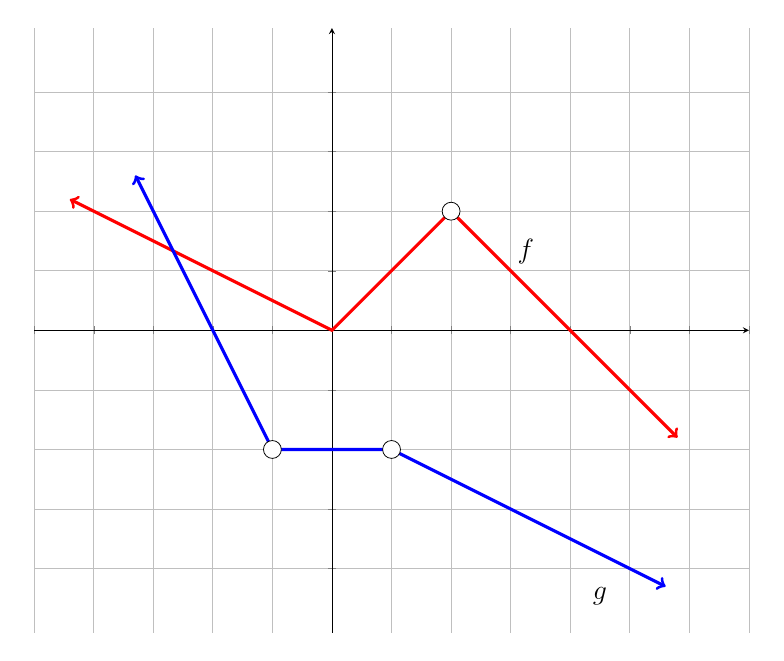
\begin{tikzpicture}[scale=.7]
      \begin{axis}[
        \usualgrid{-5}{7}{-4}{4}
        disabledatascaling,
        width=1.2\textwidth,
        axis equal,
        ]
                \draw[<->,ultra thick,red] (-4.4,2.2) -- (0,0) -- (2,2) -- (4,0) -- (5.8,-1.8);
        \draw[fill=white] (2,2) circle (0.15);
        \node[above right] at (3,1) {\Large{$f$}};

        \draw[<-,ultra thick,blue] (-3.3,2.6) -- (-1,-2) -- (1,-2);
        \draw[->,ultra thick,blue] (1,-2) -- (5.6,-4.3);
        \draw[fill=white] (-1,-2) circle (0.15);
        \draw[fill=white] (1,-2) circle (0.15);
        \node [below] at (4.5,-4.2) {\Large{$g$}};
        
       \end{axis}
    \end{tikzpicture}
\end{center}

\begin{enumerate}
\item Find the domain and range of $f(x)$. 
\item Find where $f(x)$ is increasing, where it's decreasing, and where it's constant, if any.
\item Find the domain and range of $g(x)$.
\item Find where $g(x)$ is increasing, where it's decreasing, and where it's constant, if any.
\item Find the $x$ and $y$ intercepts of $g(x)$, if they exist. 
\item Find the $x$ and $y$ intercepts of $f(x)$, if they exist. 
\item Find where $f(x)>1$. 
\item Find where $g(x)\geq 0$. 
\item Find the relative minimum and maximum of $g(x)$ if it exists.
\item Find the relative minimum and maximum of $f(x)$ if it exists.
\item Find the domain of $(f\circ g)(x)$. 
\item Find the domain of $(g\circ f)(x)$. 
\item Determine whether $f(x)$ is 1-1. Justify your answer. If it is 1-1, sketch the graph of $f^{-1}(x)$.
\item Determine whether $g(x)$ is 1-1. Justify your answer. If it is 1-1, sketch the graph of $g^{-1}(x)$. 
\item Find $(f\circ g)(0)$. 
\item Find $(f+g)(3)$.
\item Find the domain of $(f+g)(x)$.
\item Find $\displaystyle \left(\frac{f}{g}\right)(5)$. 
\item Find the domain of $\displaystyle \left(\frac{f}{g}\right)(x)$.
\item Find the domain and range of $-2f(1-x)$, and sketch a graph. 
\item Find the domain and range of $g(2x)-1$ and sketch a graph. 
\item Find the domain and range of $g(\sqrt{x})$.
\item Describe $f(x)$ and $g(x)$, using a piecewise defined function. 
\end{enumerate}




\item Some information about the functions $f$ and $g$ are given below.

For the function $f(x)$:
\begin{itemize}
\item Domain: $[-1, \infty)$.
\item Range: $(-10, \infty)$.
\item $f(x)$ is 1-1.
%\item $f(x)$ has a horizontal asymptote at $y=-10$.
\item The following tables give some selected ordered pairs for the function $f$. 
\noindent
\begin{center}
\begin{tabularx}{400pt}{*{6}{|>{\centering\arraybackslash}X}|}
\hline
$x$ & 9 & 4 & 6& 12 & 3\\
\hline
$f(x)$& 6 & -3& 7& 5&9\\
\hline
\end{tabularx}
\end{center}
\end{itemize}


For the function $g(x)$:
\begin{itemize}
\item Domain: $(-\infty, -3)\cup(-3, \infty)$
\item Range: $[0, \infty)$
%\item $g(x)$ has a vertical asymptote at 
\item The following tables give some selected ordered pairs for the functions $g$, 
\noindent
\begin{center}
\begin{tabularx}{400pt}{*{6}{|>{\centering\arraybackslash}X}|}
\hline
$x$ & 2 & 7 & 1& 9 & 5\\
\hline
$g(x)$& 3 & 4& 9&12&6\\
\hline
\end{tabularx}
\end{center}
\end{itemize}

Answer the following questions: 
\begin{enumerate}
\item Find $(f\circ g)(1)$.
\item Find $(f\circ g)(7)$. 
\item Find $(g\circ f)(12)$
\item Find $(g\circ f)(6)$. 
\item Find $(g\circ g)(1)$.
\item Find  $(f\circ f\circ f)(3)$. 
\item Find $(f+g)(9)$.

\item Does $f(x)$ have an inverse $f^{-1}(x)$? Justify your answer. If the inverse exists, find the domain and range of $f^{-1}(x)$ and find a similar table of ordered pairs for $f^{-1}(x)$. 
\item Find $f^{-1}(6)$.
\item Does $g(x)$ have an inverse $g^{-1}(x)$? Justify your answer. If the inverse exists, find the domain and range of $g^{-1}(x)$ and find a similar table of ordered pairs for $g^{-1}(x)$.
\item Does $f(x)$ have an $y$-intercept? Justify your answer. Can $f(x)$ have more than one $y$-intercept? Justify your answer.
\item Does $f(x)$ have an $x$-intercept? Justify your answer. Can $f(x)$ have more than one $x$-intercept? Explain why or why not.
\item Does $g(x)$ have an $y$-intercept? Justify your answer. Can $g(x)$ have more than one $y$-intercept? Explain why or why not.
\item Does $g(x)$ have an $x$-intercept? Justify your answer. Can $g(x)$ have more than one $x$-intercept? Explain why or why not.
\item Find the domain $(f\circ g)(x)$.
\item Find the domain of $(g\circ f)(x)$. 

\item Find the domain and range of $\displaystyle \frac{1}{2}g(x+1)-1$, and a similar table of ordered pairs.
\item Find the domain and range of $-f(3x)+2$, and a similar table of ordered pairs. Is $-f(3x)+2$ still a 1-1 function?
\item Suppose $f(a^2-3)=7$. Can you find all possible values of $a$? Explain why or why not. If it's possible, find all such values. 
\item Suppose $g(t-1)=12$. Can you find all possible values of $t$? Explain why or why not. If it's possible, find all such values.
\end{enumerate}

\item \textit{(Hard/Challenge)} For the functions below, $a$, $b$, $m$, and $n$ are all real valued constants. 
\begin{enumerate}
\item Consider $f(x)=mx+b$. Determine all values of $m$ and $b$ that makes $f(x)$ a 1-1 function. Write down an expression for $f^{-1}(x)$ in those cases using $m$ and $b$. 
\item Consider $\displaystyle g(x)=\frac{ax+b}{mx+n}$. Determine all values of $a, b, m,$ and $n$ that make $g(x)$ a 1-1 function. Write down an expression for $g^{-1}(x)$ in those cases using $a, b, m$ and $n$.
\item Consider $h(x)=\frac{1}{ax^2+b}$. 
\begin{itemize}
\item Find the values of $a$ and $b$ so that $h(x)$ is not a function.
\item For all values of $a$ and $b$, $h(x)$ is not a 1-1 function. Explain why not.
\item Find the values of $a$ and $b$ so that $h(x)$ is a constant function. 
\item In most cases of $a$ and $b$, $h(x)$ is a non-constant function. It is possible in those situations to restrict the domain of $h(x)$ so that it is 1-1. Find the necessary restriction on the domain, and find the inverse. 
\end{itemize}  
\end{enumerate}



\end{enumerate}
\end{document}

\end{document}